%%%%%%%%%%%%%%%%%
% W tagging
%%%%%%%%%%%%%%%%%

In order to identify boosted $\W$ bosons,  we cluster jets  with \textsc{FastJet} using the
Cambridge-Aachen algorithm~\cite{Dokshitzer:1997in} and a size parameter of 0.8, yielding CA8 jets. 
Jet energy corrections for these jets are derived from the anti-$k_\textrm{T}$ jets with  size
parameter $\Delta R=0.7$. Simulations show that the corrections are valid for CA8 jets and have an
additional uncertainty no greater than  2\%.  We require the CA8 jet mass to lie within the $\W$
boson mass range $70 < m_{jet} < 100$~\GeV and call such jets ``mass-tagged" ($Y$).  
The jet mass is calculated from the constituents of the jet after jet pruning, which removes the
softest constituents of the jet.  During jet pruning, the jet constituents are reclustered, and at
each step the softer and larger-angle ``protojet'' among the two protojets to be merged, when
failing certain criteria, is removed~\cite{Ellis:2009su,Ellis:2009me}.  
A CMS study has shown that jet pruning reduces pileup effects and provides good boosted $\W$ jet to
quark/gluon jet discrimination~\cite{Chatrchyan:2013vbb}.
Given $N$ candidate subjets, obtained with \textsc{FastJet} via exclusive $k_T$ clustering with a
one-pass optimization, in a given CA8 jet, the N-subjettiness~\cite{Thaler:2010tr} is computed
as follows, 
\begin{equation}
\tau_N = \frac{1}{R_0} \sum_k p_{T, k} \min (\Delta R_{1,k}, \Delta R_{2,k}, ... \Delta R_{N,k}) /
\sum_{k} p_{T, k},
\end{equation}
where $R_0$ is the original jet size parameter and $k$ runs over all constituent particles.  
The quantity $\tau_N$ is small if the original jet is consistent with having $N$ subjets.  
Therefore, in order to discriminate boosted $\W$ bosons, which have two subjets, from q/g jets,
characterized by a single subjet, we require $\tau_2 / \tau_1 < 0.5$.  The complement of this
selection defines anti-tagged $\W$ jets ($aW$), which are used in the definition of control regions
that are used in the background modelling.


\begin{figure}
  \centering
  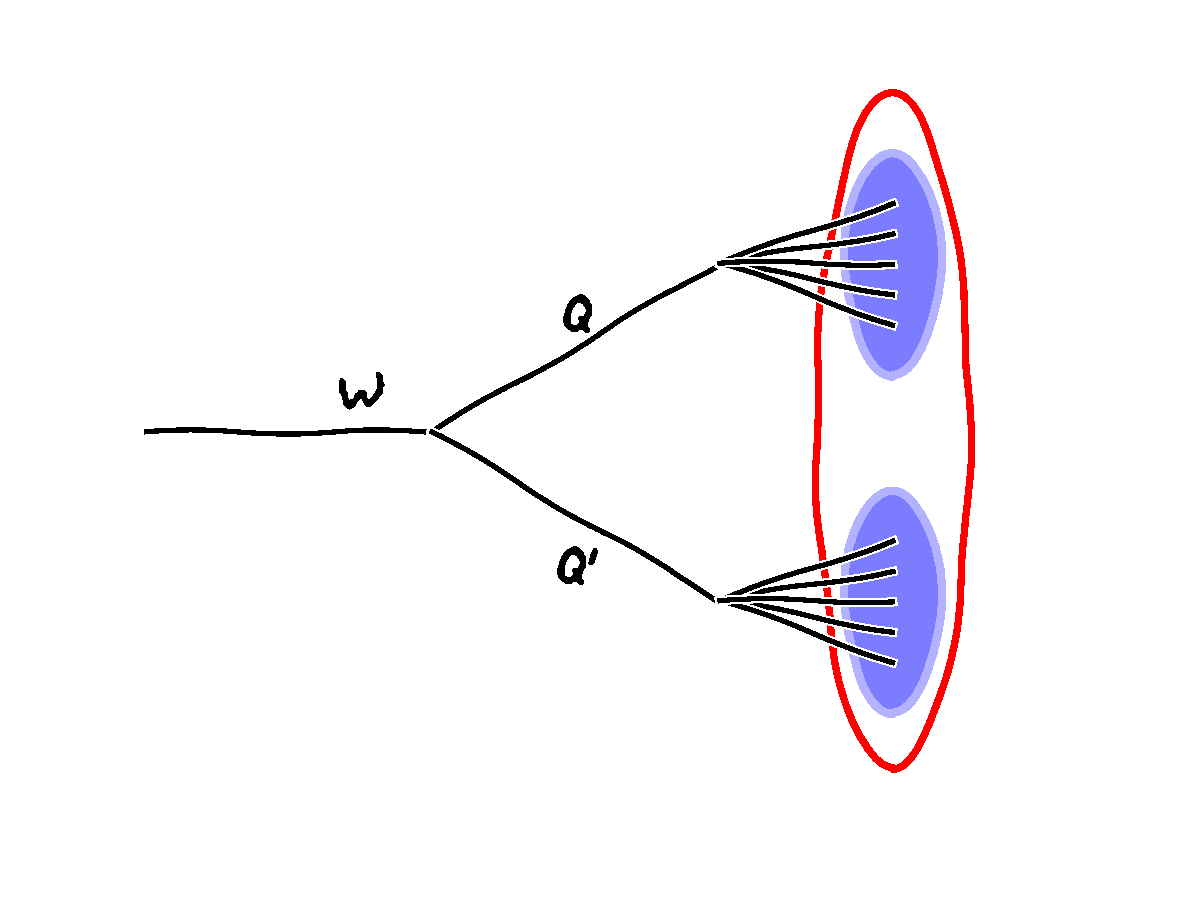
\includegraphics[width=0.48\textwidth]{figures/razor_wtag/W_subjets}
  ~
  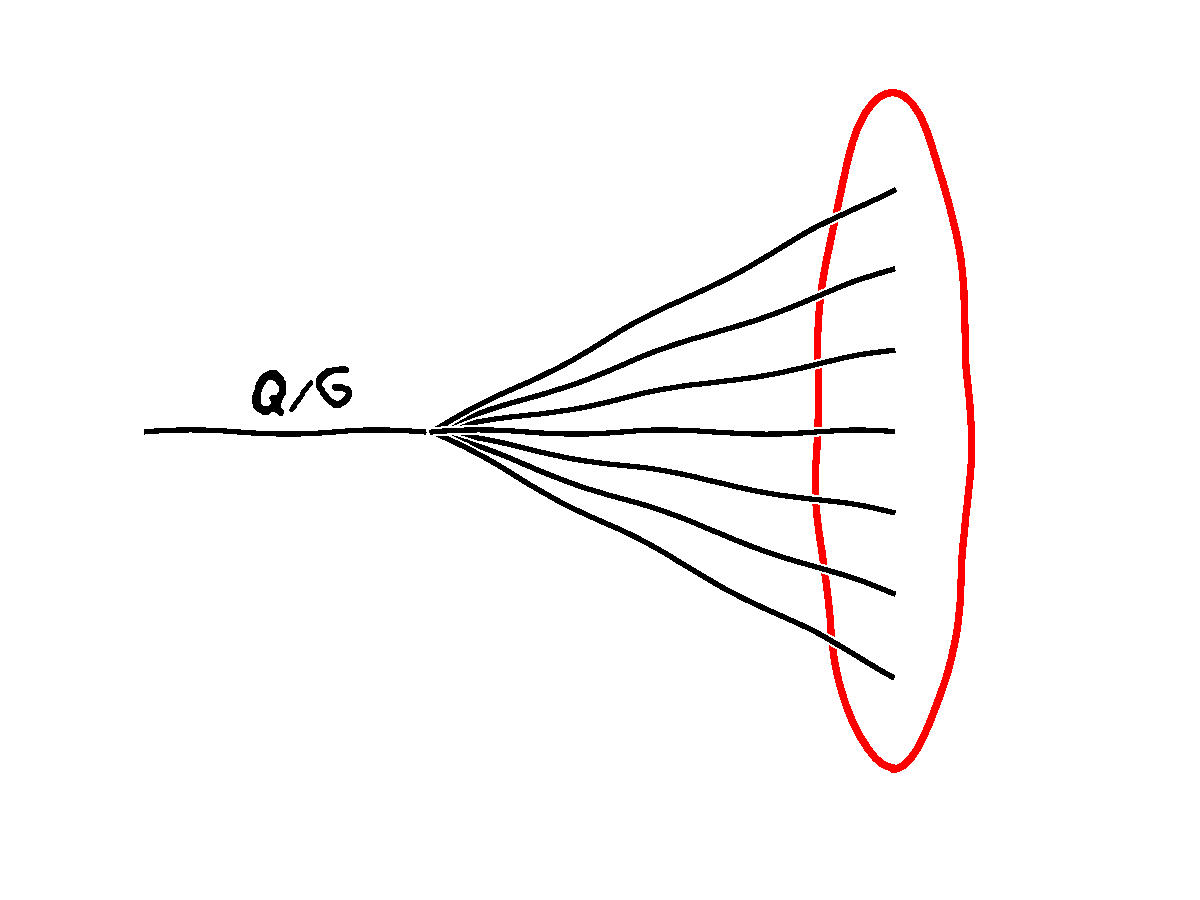
\includegraphics[width=0.48\textwidth]{figures/razor_wtag/qg_jets}
  \caption{The jet substructure of a $\W$-initiated jet differs from a q/g-initiated jet.
  \label{fig:boost_wtag_cartoon}}
\end{figure}
